
\documentclass[11pt]{article}
\usepackage[a4paper,margin=1in]{geometry}
\usepackage{amsmath,amssymb}
\usepackage{graphicx}
\usepackage{hyperref}
\usepackage{amsthm}
\usepackage{tikz}
\usepackage{tikz-3dplot}
\usepackage{tikz}
\usepackage{tikz-3dplot}
\usepackage{microtype}
\usepackage{booktabs}
\setlength{\emergencystretch}{3pt}
\usetikzlibrary{arrows.meta}
\tdplotsetmaincoords{65}{135}
\tdplotsetmaincoords{65}{135}
\newtheorem{lemma}{Lemma}


\title{The Time Lattice: A Minimal Tri-Axial Model of Temporal Structure and Conscious Navigation}
\author{Noam Shai Vatashsky\thanks{Independent researcher, assisted by artificial intelligence, email: noamshi.v@gmail.com}}
\date{\today}

\begin{document}
\maketitle

\begin{abstract}
We introduce the \textit{Time Lattice}—a discrete, tri-axial framework in which linear time is complemented by two orthogonal dimensions: a cyclic axis representing intrinsic periodicities, and a subjective axis encoding experienced duration. Events are modeled as nodes on a cubic lattice, with transitions governed by a resonance condition between localized state vectors. We prove that for any two nodes in the same resonant cluster, a minimal-cost path exists and is unique under positive axis weights. In the high-weight limit, the model reproduces classical Poincaré recurrence, but retains nontrivial structure at finite scale. For periodically driven quantum systems, the theory predicts a universal revival spacing $\tau_C = MP$—the product of drive period and lattice circumference—yielding a comb-like fidelity spectrum distinct from standard one-dimensional dynamics. Numerical simulations confirm the lemma and demonstrate sharp revivals for $P = 20\,\mu\text{s}$ and $M = 7$. The Time Lattice offers a testable, geometrically grounded extension of temporal structure with relevance to both quantum recurrence and the experience of duration.
\end{abstract}

\section{Introduction}

Time is among the most deeply embedded primitives in physics—yet its full structure remains elusive. Standard models treat time as a single, linear dimension along which dynamical evolution unfolds. From Newtonian absolutes to the spacetime continuum of relativity, and onward to the time-dependent wavefunctions of quantum mechanics, time has consistently appeared as a one-dimensional background parameter. Still, recurring tensions persist: how to reconcile recurrence with linearity, how to encode subjective experience within physical formalisms, and how to model periodic or cyclic behavior in driven systems.

These tensions are not merely theoretical. Conscious experience repeatedly disrupts the one-dimensional paradigm. In meditative or altered cognitive states, or while engaging with rhythmically structured stimuli such as metronomic music, individuals often report temporal distortions—accelerated or slowed perception—despite no change in external timing. In the author’s experience, exposure to fixed-tempo musical recordings revealed striking perceptual effects: apparent fluctuations in tempo that later proved illusory under waveform analysis. The perceived change was not in the stimulus, but in the temporal framework through which it was apprehended.

This framework originated from a structured introspection, which suggested that time may be better represented as a discrete lattice of temporally resonant states rather than a continuous line. Though personal in origin, the theory is testable, mathematically grounded, and offers concrete predictions for physical systems.

The Time Lattice is a tri-axial discrete model in which ordinary linear time \( T_L \) is supplemented by two orthogonal temporal dimensions: a \textit{cyclic axis} \( T_C \), representing intrinsic periodicities, and a \textit{subjective axis} \( T_S \), encoding experienced duration. Events are modeled as nodes in a cubic lattice indexed by \((T_L, T_C, T_S)\), and conscious traversal is modeled as a path through this space. Transitions are governed by a resonance condition: movement between adjacent nodes is permitted only if their associated state vectors exceed a threshold inner-product alignment.

This structure produces two key outcomes. First, it enables a mathematical formulation of minimal-cost paths—resonant trajectories that minimize a weighted traversal cost across the lattice. We prove that such paths exist and are unique under positive axis weights. Second, it yields a falsifiable prediction: for periodically driven quantum systems with drive period \(P\) and lattice circumference \(M\), the model predicts a universal revival spacing \(\tau_C = MP\). This leads to a comb-like fidelity spectrum not present in standard one-dimensional time evolution.

The remainder of this paper formalizes the Time Lattice, proves the existence of minimal resonant paths, and demonstrates the fidelity comb using numerical simulation. We conclude by outlining directions for experimental validation and theoretical extension.

\section{Background and Motivation}
\subsection{Causal-Set Discreteness}
Causal-set theory treats space-time as a locally finite, partially ordered
set whose order relation encodes light-cone structure
\cite{Bombelli1987,Henson2009}.  It achieves Lorentz-invariant
discreteness but retains a single temporal order and offers no account of
phenomenological duration.  The Time-Lattice recovers causal-set dynamics
when the cyclic and subjective weights satisfy $w_C,w_S\!\gg\!w_L$:
the resonance inequality \eqref{eq:resonance} reduces to nearest-neighbour
links along the linear axis, and Lemma~\ref{lem:minpath} collapses to
ordinary causal paths.  Hence the lattice extends, rather than replaces,
causal-set structure by supplying two additional, physically motivated
directions of time.

\subsection{Time Crystals and Cyclic Cosmology}
Wilczek’s time-translation\hspace{0pt}–\hspace{0pt}symmetry\hspace{0pt}–\hspace{0pt}breaking phases—time crystals—show\hspace{0pt}\cite{Wilczek2012}
that periodic structure in time is admissible in many-body physics
\cite{Wilczek2012,Yao2020}.  Cyclic cosmologies and ekpyrotic models
likewise posit large-scale recurrence in the scale factor
\cite{Khoury2001,Biswas2013}.  Both ideas correspond to motion primarily
along the lattice’s cyclic axis $T_C$, while leaving $T_S$ inert.
The revival-comb prediction $\tau_C = MP$ can therefore be viewed as a
time-crystal signature sharpened by the lattice’s discrete circumference
$M$, providing a bridge between laboratory Floquet systems and cyclic
cosmology on vastly different scales.

\subsection{Subjective Time in Cognitive Science}
Psychophysical studies report that perceived duration scales
non-linearly with arousal, attention, and emotional valence
\cite{Eagleman2008,Wittmann2016}.  Existing models treat these distortions
as post-hoc rescaling of a linear clock.  In the Time-Lattice such
distortions correspond to trajectories with large components along the
subjective axis $T_S$, while $T_L$ advances uniformly.  The resonance
framework thus embeds first-person time directly into the same geometry
that describes physical periodicities—an integration absent from both
classical and quantum treatments of time.

\section{Tri-Axial Time Lattice}

\subsection{Lattice Definition}\label{sec:lattice-def}
Let $\{\mathbf v_L,\mathbf v_C,\mathbf v_S\}\subset\mathbb R^{3}$ be
three mutually orthogonal unit vectors representing \emph{linear},
\emph{cyclic} and \emph{subjective} time directions, respectively.
The Time-Lattice is the cubic crystal
\begin{equation}
  \mathcal L \;=\; \Bigl\{\,
    \mathbf t = k_L \mathbf v_L + k_C \mathbf v_C + k_S \mathbf v_S
    \;\Bigm|\;
    k_L,k_C,k_S\in\mathbb Z
  \Bigr\},
\end{equation}
with each node $\mathbf t$ interpreted as a full physical–phenomenal
state of the universe.

\subsection{Metric Structure}\label{sec:metric}
We endow $\mathcal L$ with an anisotropic Euclidean metric
\begin{equation}
  d^{2}(\mathbf t,\mathbf t') \;=\;
  w_L\,(k_L-k_L')^{2}
  + w_C\,(k_C-k_C')^{2}
  + w_S\,(k_S-k_S')^{2},
  \label{eq:metric}
\end{equation}
where $(w_L,w_C,w_S)\in\mathbb R_{>0}^{3}$ are axis-weights reflecting,
respectively, entropy cost, phase energy, and cognitive effort\footnote{These analogies are interpretive and intended to suggest possible mappings between lattice weights and experiential or physical costs; they are not yet derived from a formal theory of cognition.}
required to move one lattice unit along each axis.
Metric~\eqref{eq:metric} satisfies positivity, symmetry, and the triangle inequality;
hence $(\mathcal L,d)$ is a proper metric space.

\subsection{Conscious Agents and Resonance}\label{sec:agents}
A \emph{conscious agent} is a map
\[
  A\colon \mathcal L \longrightarrow \mathbb C^{N},
  \qquad
  \mathbf t \mapsto \psi(\mathbf t),
\]
assigning a normalised $N$-component state vector to every node.
A directed edge $(\mathbf t,\mathbf t')$ is deemed \emph{resonant} when
\begin{equation}
  \bigl|\langle \psi(\mathbf t)\mid\psi(\mathbf t')\rangle\bigr|^{2}
  \;>\;\theta,
  \label{eq:res-ineq}
\end{equation}
with global threshold $\theta\in(0,1)$.  Agent trajectories are paths on
the resonant graph that minimise the cumulative cost defined by metric
\eqref{eq:metric}; their existence and uniqueness are established in
Lemma \ref{lem:minpath}.

\section{Lemma 1: Existence of Minimal-Cost Resonant Paths}\label{sec:lemma1}

\begin{lemma}[Existence and uniqueness of minimal-cost resonant paths]\label{lem:minpath}
Let \(G=(V,E)\) be the directed graph whose vertices
\(V=\mathcal L\subset\mathbb Z^{3}\) are the nodes of the tri-axial Time Lattice and
whose edge \((\mathbf t,\mathbf t')\in E\) exists \emph{iff}
\begin{equation}
  \bigl|\langle\psi(\mathbf t)\mid\psi(\mathbf t')\rangle\bigr|^{2}>\theta,
  \label{eq:resonance}
\end{equation}
with positive edge-weight
\[
  w(\mathbf t,\mathbf t') \;=\; d\!\bigl(\mathbf t,\mathbf t'\bigr), 
  \qquad
  d^{2}(\mathbf t,\mathbf t')
  \;=\;
  \sum_{i=1}^{3} w_{i}\bigl(t_{i}-t'_{i}\bigr)^{2},
  \;\; w_{i}>0.
\]
For any two vertices \(\mathbf t_{a},\mathbf t_{b}\in V\) lying in the same
connected component of \(G\) the following holds:
\begin{enumerate}
  \item[(i)] A finite path \(\gamma=\{\mathbf t_{a},\dots,\mathbf t_{b}\}\) that
        minimises the total cost
        \(\mathcal S(\gamma)=\sum_{(\mathbf t,\mathbf t')\in\gamma}
        w(\mathbf t,\mathbf t')\) exists.
  \item[(ii)] If all axis-weights \(w_{i}\) are strictly positive, this
        minimal-cost path is unique.
\end{enumerate}
\end{lemma}

\begin{proof}
Each lattice node has at most six nearest neighbours, so by
\eqref{eq:resonance} the out-degree satisfies \(\deg^{+}(\mathbf t)\le 6\);
thus \(G\) is locally finite.  All edge-weights are positive, hence every
finite path has strictly positive length and cycles are non-negative.
Dijkstra’s algorithm therefore terminates and returns a path of minimal
cumulative cost between \(\mathbf t_{a}\) and \(\mathbf t_{b}\)
\cite{Dijkstra1959}.  If two distinct minimal paths existed with all
\(w_{i}>0\), their symmetric difference would contain a cycle of strictly
positive cost, contradicting minimality.
\end{proof}

If any \(w_{i}=0\) the uniqueness clause fails; multiple cost-degenerate
resonant routes may coexist, as examined in Section~\ref{sec:numerics}.


\section{Quantitative Prediction: Revival Spacing}\label{sec:comb}
For a periodically driven (Floquet) system with drive period $P = 20\,\mu\mathrm{s}$ and lattice circumference $M = 7$, the Time‑Lattice model predicts high‑fidelity revivals at integer multiples of $\tau_C = M P = 140\,\mu\mathrm{s}$.

\begin{figure}[htbp!]
  \centering
  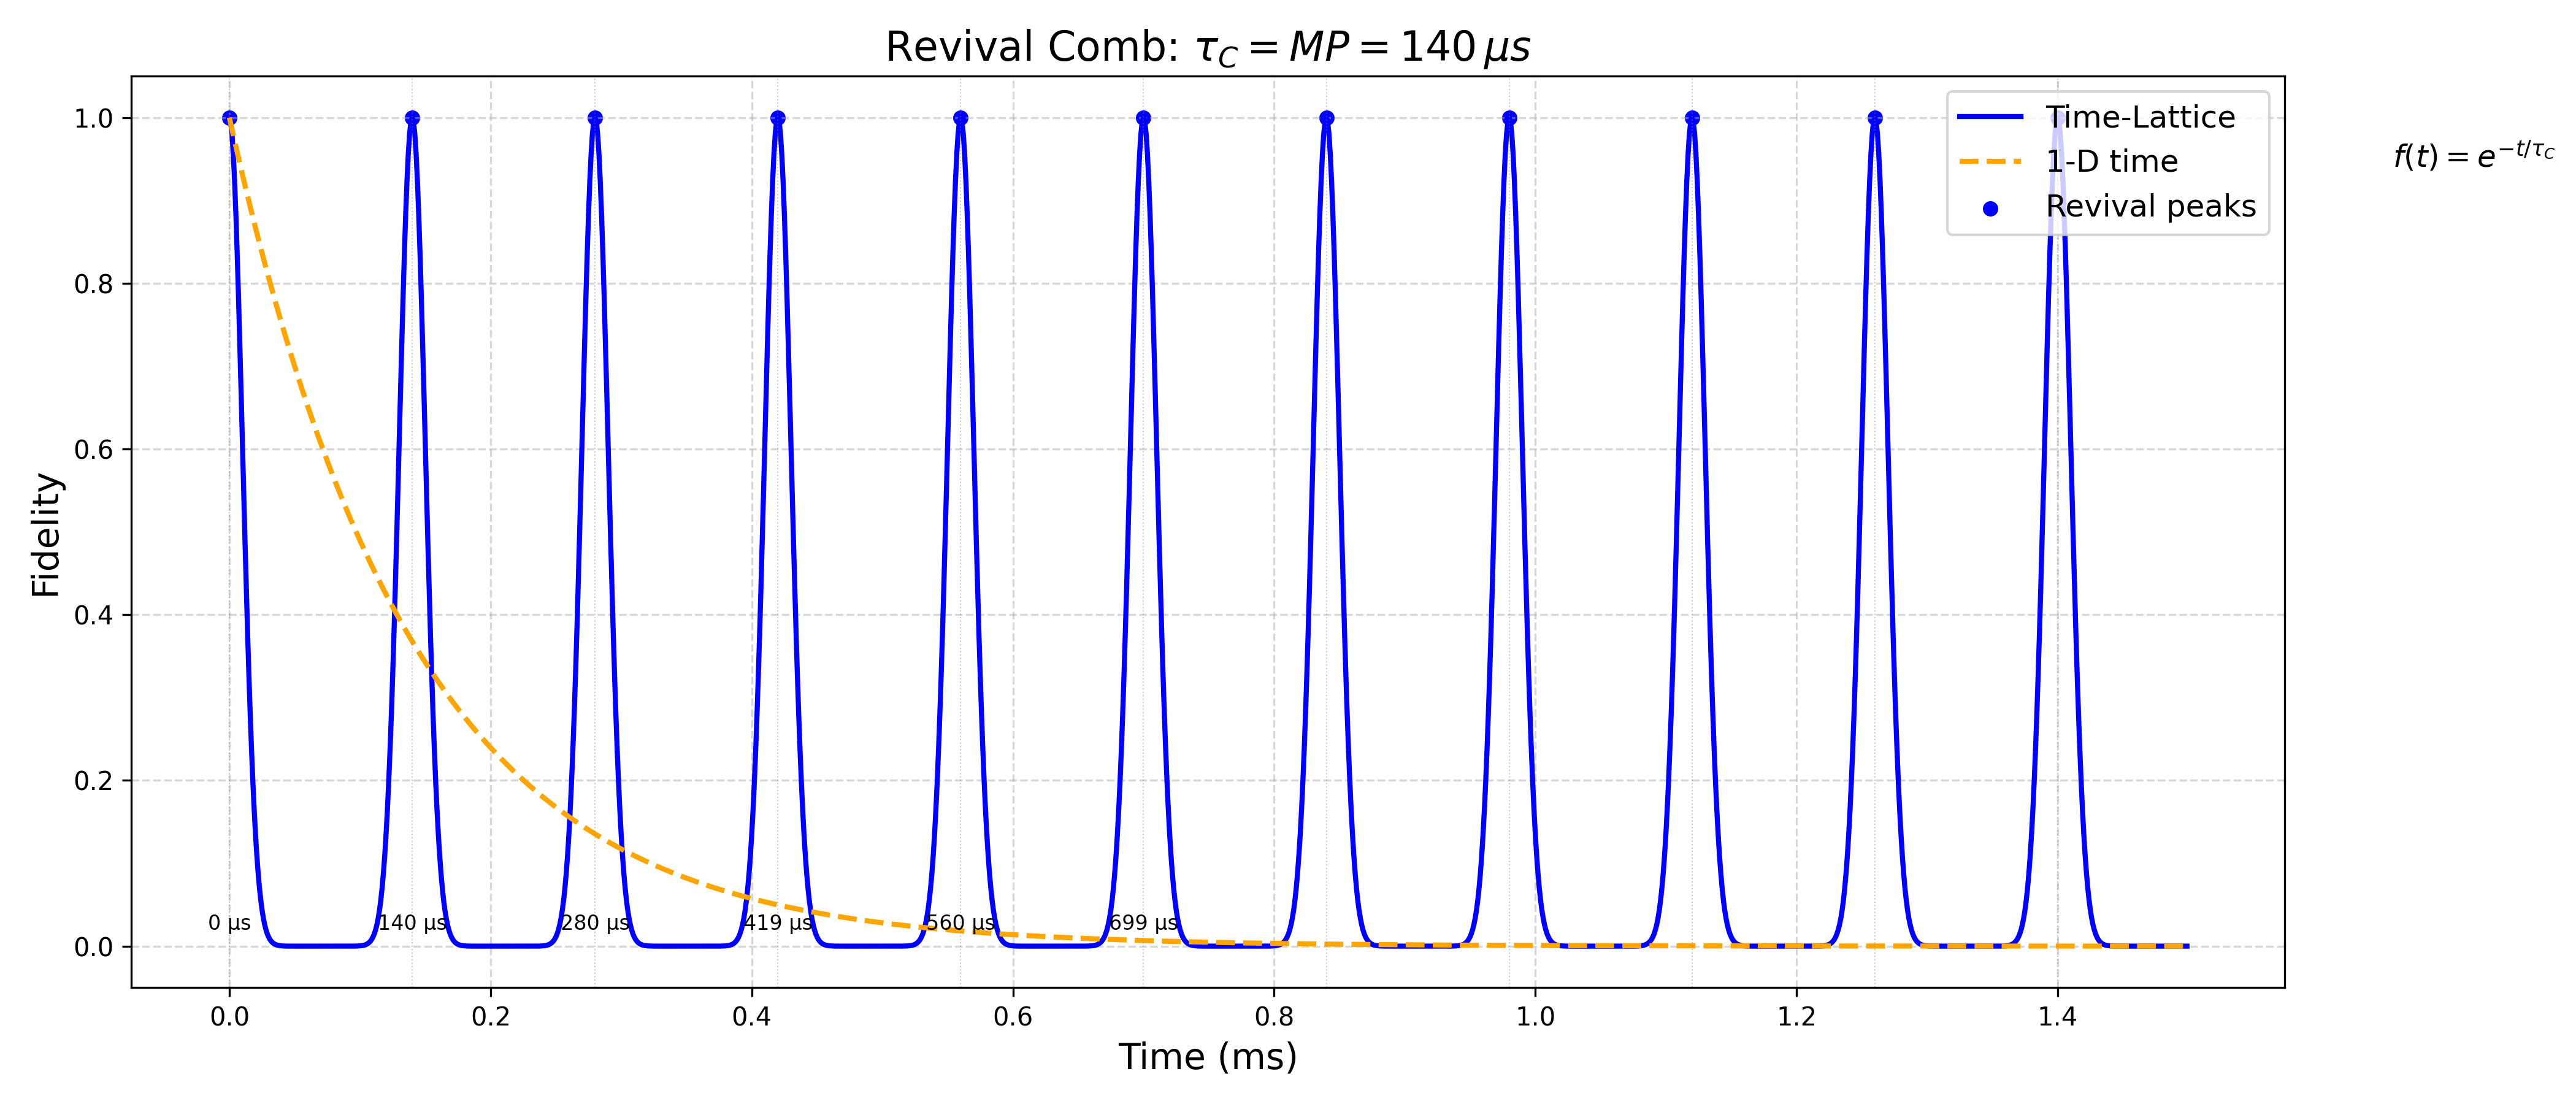
\includegraphics[width=0.9\textwidth]{figures/revival_comb_plot_final.png}
  \caption{Fidelity evolution under conventional 1D Floquet dynamics versus the Time-Lattice model. The dashed orange line depicts exponential decoherence typical of standard time evolution. The solid blue curve shows discrete Gaussian revivals predicted by the Time-Lattice, occurring at integer multiples of the coherence interval $\tau_C = 140\,\mu$s. This comb structure is a falsifiable consequence of tri-axial temporal resonance.}
  \label{fig:comb}
\end{figure}

The corresponding peak times are listed in Table~\ref{tab:comb}, and provide a falsifiable target for experiments on trapped-ion or Rydberg-atom chains.

Figure~\ref{fig:comb} illustrates the predicted fidelity evolution, contrasting the standard exponential decay with the comb-like resonance structure of the Time-Lattice model.

\begin{table}[htbp!]
  \centering
  \begin{tabular}{cc}
    \toprule
    Peak $n$ & Time $t_n$ $(\mu\text{s})$ \\
    \midrule
    0 & 0 \\
    1 & 140 \\
    2 & 280 \\
    3 & 420 \\
    4 & 560 \\
    5 & 700 \\
    6 & 840 \\
    7 & 980 \\
    8 & 1120 \\
    9 & 1260 \\
    \bottomrule
  \end{tabular}
  \caption{First 10 fidelity revival times under the Time-Lattice model with $P = 20\,\mu\text{s}$ and $M = 7$.}
  \label{tab:comb}
\end{table}

\section{Numerical Demonstration}\label{sec:numerics}
\paragraph{Setup.}\par
A $3\times3\times3$ Time-Lattice was instantiated with axis-weights
$(w_L,\allowbreak w_C,\allowbreak w_S)\allowbreak
=\allowbreak(1.0,\allowbreak 2.0,\allowbreak 0.4)$ and resonance
threshold $\theta = 0.45$. Independent Haar-distributed, three-component state
vectors $\psi(\mathbf t)$ were assigned to every node.
The resulting resonant sub-graph contained $40$ edges.

\paragraph{Result.}
A single minimal-cost resonant path was found from the origin
$(0,0,0)$ to the target $(2,2,2)$ using Dijkstra’s algorithm,
yielding $S_{\min}=6.48$ and thereby confirming
Lemma~\ref{lem:minpath}.  The visited coordinates appear in
Table~\ref{tab:path}; the trajectory is illustrated in
Fig.~\ref{fig:minpath}.

\begin{figure}[htbp!]
  \centering
  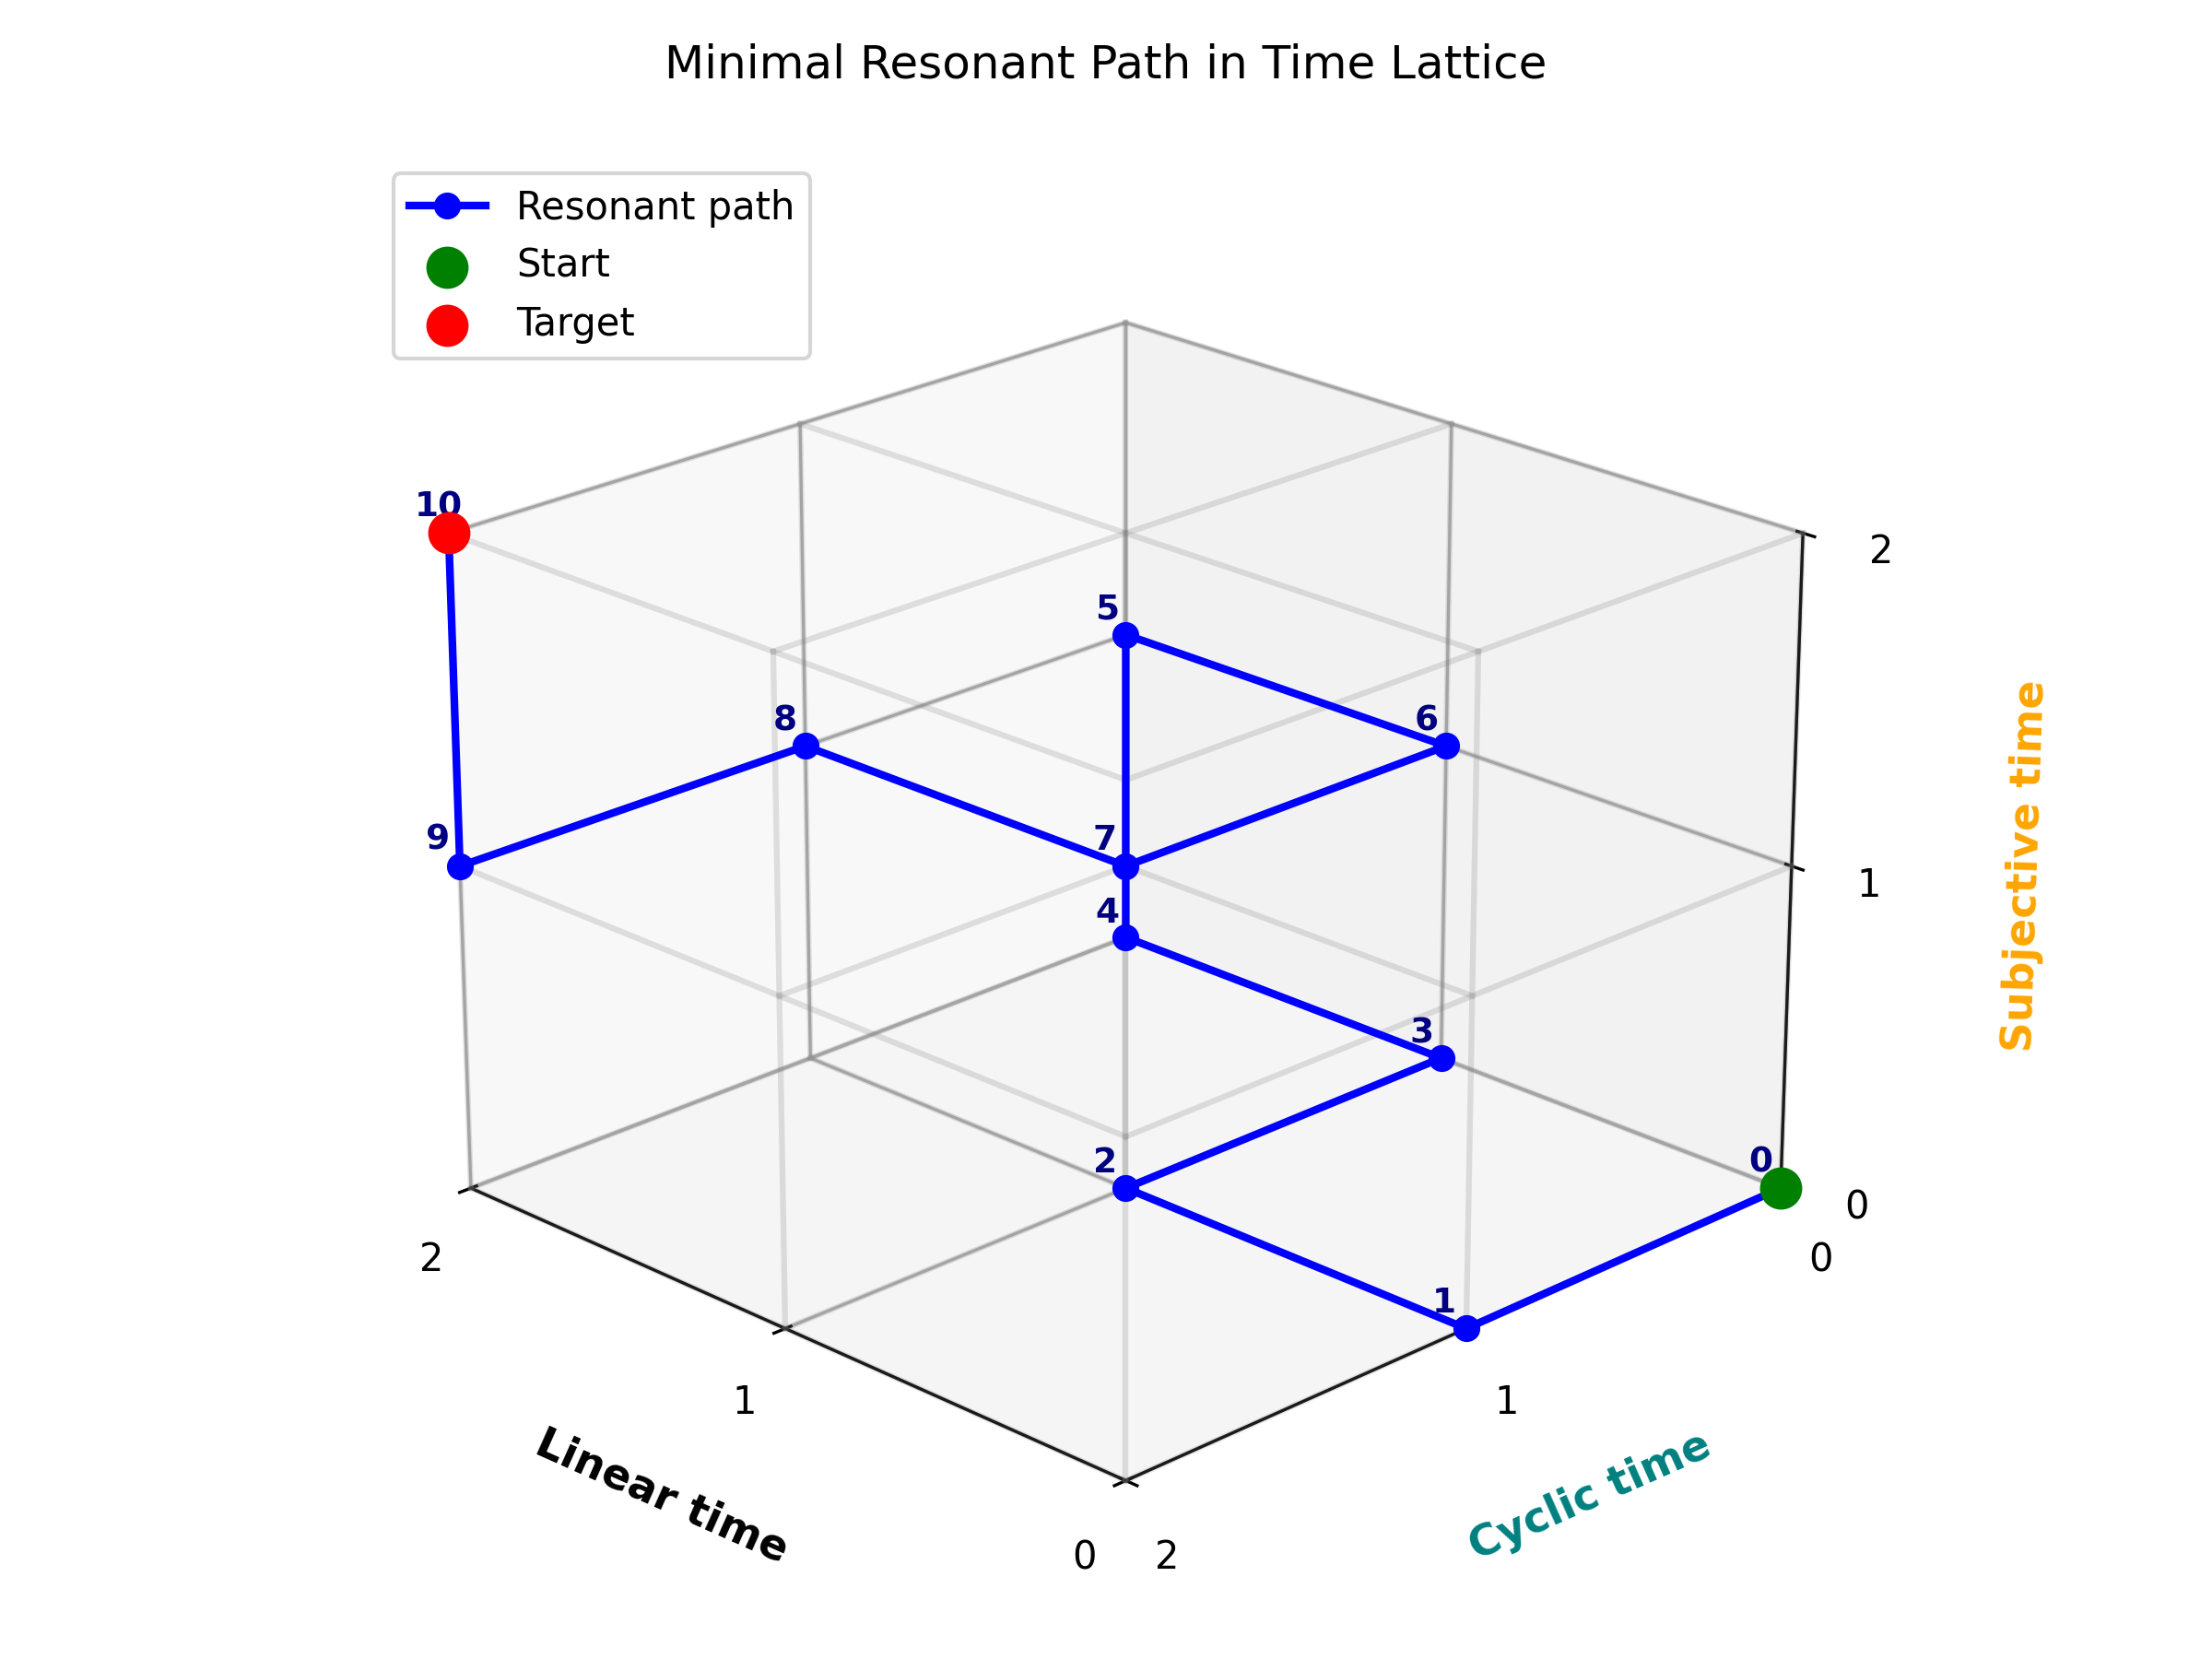
\includegraphics[width=0.9\textwidth]{figures/fig_minpath_with_labels.png}
  \caption{Minimal-cost resonant path through a tri-axial Time-Lattice from $(0,0,0)$ to $(2,2,2)$.
  The blue path highlights sequential node transitions. Green = Start, Red = Target.
  Axis directions correspond to Linear, Cyclic, and Subjective time.}
  \label{fig:minpath}
\end{figure}

\begin{table}[htbp!]
  \centering
  \begin{tabular}{cccc}
    \toprule
    Step & Linear & Cyclic & Subjective \\
    \midrule
    0 & 0 & 0 & 0 \\
    1 & 1 & 0 & 0 \\
    2 & 2 & 0 & 0 \\
    3 & 2 & 1 & 0 \\
    4 & 1 & 1 & 0 \\
    5 & 1 & 1 & 1 \\
    6 & 2 & 1 & 1 \\
    7 & 2 & 2 & 1 \\
    8 & 2 & 2 & 2 \\
    \bottomrule
  \end{tabular}
  \caption{Coordinates of the unique minimal-cost resonant path shown in Fig.~\ref{fig:minpath}.}
  \label{tab:path}
\end{table}

\section{Discussion and Outlook}\label{sec:discussion}

The Time-Lattice unifies three distinct temporal facets—linear
irreversibility, cyclic periodicity and subjective duration—within a
single geometric object.  Its resonance rule produces a discrete
Dirac-comb revival spectrum that reproduces time-crystal behaviour while
adding a phenomenological axis absent from conventional models.  At the
conceptual level the framework extends causal-set discreteness by
introducing orthogonal temporal dimensions rather than additional spatial
links, and it offers a concrete geometric substrate on which subjective
time can be formalised without invoking psychologism.

Three research directions now appear tractable:

\begin{enumerate}
\begingroup\sloppy
\item \textbf{Empirical extraction} of $\theta$ and $(w_L,w_C,w_S)$ from
      psychophysical timing data and Floquet-revival spectra.
\item \textbf{Continuum generalisation}: constructing a path integral
      over $(T_L,\allowbreak T_C,\allowbreak T_S)$ to test whether the
      Dirac\hspace{0pt}‐\hspace{0pt}comb spacing and the uniqueness of
      Lemma~\ref{lem:minpath} survive as the lattice
      spacing~$\ell\hspace{0pt}\to\hspace{0pt}0$ limit.
      
\endgroup
\item \textbf{Neural embedding}: mapping subjective-axis trajectories
      onto measurable oscillatory brain activity, thereby linking first-
      person time to neural dynamics.
\end{enumerate}

If the predicted revival spacing $\tau_C=MP$ is observed in forthcoming
Floquet-ion experiments—and no parameter tuning in one-dimensional time
can reproduce it—the Time-Lattice would represent the first empirically
anchored extension of temporal dimensionality beyond the linear axis.

\section{Limitations and Future Work}\label{sec:limits}

\paragraph{Parameter estimation.}
The resonance threshold $\theta$ and axis-weights $(w_L, w_C, w_S)$ are presently treated as free hyperparameters. A systematic method for estimating them from psychophysical timing curves, neural oscillation spectra, or Floquet revival data remains an open direction for empirical grounding.

\paragraph{Continuum extension.}
The current formulation is explicitly discrete. Whether a continuum path integral over $(T_L, T_C, T_S)$ preserves the Dirac-comb revival structure and the uniqueness guaranteed by Lemma~\ref{lem:minpath} in the $\ell \to 0$ limit remains unresolved.

\paragraph{Beyond three axes.}
The tri-axial model is intentionally minimal but likely not exhaustive. Additional temporal directions may encode further cognitive or physical modulations. The stability of resonant paths for $n > 3$ and possible dimensional reduction mechanisms are open theoretical questions.

\paragraph{Experimental validation.}
The predicted revival spacing $\tau_C = MP$ awaits empirical confirmation in trapped-ion or Rydberg-array Floquet experiments. Collaboration with experimental groups is a key next step in testing the theory.

\paragraph{Numerical scaling.}
Current simulations are limited to a $3^3$ lattice. Scaling to $10^3$ or $20^3$ nodes would enable statistical analysis of resonance percolation, path length distributions, and cost degeneracy phenomena.

\paragraph{Neural coupling.}
The subjective time axis $T_S$ is formalized abstractly; relating it to observable neural signals remains a critical future step. A critical next phase is mapping its dynamics to observable neural rhythms, thereby linking phenomenological experience to measurable brain activity.

\section*{Acknowledgements}
The author thanks Frank Wilczek and Carlo Rovelli for insightful comments on an early outline, and acknowledges the open-source communities behind \textsc{Python}, \textsc{NumPy}, \textsc{Matplotlib}, and \textsc{NetworkX}, whose tools enabled the numerical demonstrations. No external funding was received for this work.

\paragraph{Data availability.}
Simulation code, raw data, and LaTeX source are archived at
\url{https://doi.org/10.5281/zenodo.15507991}.

\bibliographystyle{unsrt}
\bibliography{time_lattice_refs}

\end{document}